\PassOptionsToPackage{unicode=true}{hyperref} % options for packages loaded elsewhere
\PassOptionsToPackage{hyphens}{url}
%
\documentclass[]{article}
\usepackage{lmodern}
\usepackage{amssymb,amsmath}
\usepackage{ifxetex,ifluatex}
\usepackage{fixltx2e} % provides \textsubscript
\ifnum 0\ifxetex 1\fi\ifluatex 1\fi=0 % if pdftex
  \usepackage[T1]{fontenc}
  \usepackage[utf8]{inputenc}
  \usepackage{textcomp} % provides euro and other symbols
\else % if luatex or xelatex
  \usepackage{unicode-math}
  \defaultfontfeatures{Ligatures=TeX,Scale=MatchLowercase}
\fi
% use upquote if available, for straight quotes in verbatim environments
\IfFileExists{upquote.sty}{\usepackage{upquote}}{}
% use microtype if available
\IfFileExists{microtype.sty}{%
\usepackage[]{microtype}
\UseMicrotypeSet[protrusion]{basicmath} % disable protrusion for tt fonts
}{}
\IfFileExists{parskip.sty}{%
\usepackage{parskip}
}{% else
\setlength{\parindent}{0pt}
\setlength{\parskip}{6pt plus 2pt minus 1pt}
}
\usepackage{hyperref}
\hypersetup{
            pdftitle={The Software Heritage Acquisition Process - A practical guide},
            pdfborder={0 0 0},
            breaklinks=true}
\urlstyle{same}  % don't use monospace font for urls
\usepackage{listings}
\newcommand{\passthrough}[1]{#1}
\usepackage{graphicx,grffile}
\makeatletter
\def\maxwidth{\ifdim\Gin@nat@width>\linewidth\linewidth\else\Gin@nat@width\fi}
\def\maxheight{\ifdim\Gin@nat@height>\textheight\textheight\else\Gin@nat@height\fi}
\makeatother
% Scale images if necessary, so that they will not overflow the page
% margins by default, and it is still possible to overwrite the defaults
% using explicit options in \includegraphics[width, height, ...]{}
\setkeys{Gin}{width=\maxwidth,height=\maxheight,keepaspectratio}
\setlength{\emergencystretch}{3em}  % prevent overfull lines
\providecommand{\tightlist}{%
  \setlength{\itemsep}{0pt}\setlength{\parskip}{0pt}}
\setcounter{secnumdepth}{0}

% set default figure placement to htbp
\makeatletter
\def\fps@figure{htbp}
\makeatother

  %
% put gray background around verbatim text
%
% Reference
% <https://tex.stackexchange.com/questions/411194/package-soul-error-reconstruction-failed>

%\PassOptionsToPackage{table}{xcolor}
%\PassOptionsToPackage{dvipscolor}{xcolor}
\usepackage[table,dvipscolor,usenames]{xcolor}
\usepackage{soul}

\definecolor{inlineBG}{HTML}{F3F3F3}  % same as GitHub Flavored Markdown
\sethlcolor{inlineBG}

\let\OldTexttt\texttt
\renewcommand{\texttt}[1]{\sethlcolor{inlineBG}{\ttfamily\hl{\mbox{#1}}}}

%
% configure lstlisting package
%
  \lstset{ 
  backgroundcolor=\color{gray!10},   % choose the background color; you must add \usepackage{color} or \usepackage{xcolor}; should come as last argument
  basicstyle=\normalsize,        % the size of the fonts that are used for the code
  breakatwhitespace=false,         % sets if automatic breaks should only happen at whitespace
  breaklines=true,                 % sets automatic line breaking
  captionpos=b,                    % sets the caption-position to bottom
  commentstyle=\color{mygreen},    % comment style
  deletekeywords={source},         % if you want to delete keywords from the given language
  escapeinside={\%*}{*)},          % if you want to add LaTeX within your code
  emph={git,curl},
  emphstyle={\color{blue}},
  extendedchars=true,              % lets you use non-ASCII characters; for 8-bits encodings only, does not work with UTF-8
  firstnumber=1000,                % start line enumeration with line 1000
  frame=shadowbox,	                   % adds a frame around the code
  frameround=tttt,
  rulesepcolor=\color{gray},
  columns=flexible,
  keepspaces=true,                 % keeps spaces in text, useful for keeping indentation of code (possibly needs columns=flexible)
  keywordstyle=\color{blue},       % keyword style
  language=bash,                   % the language of the code
  morekeywords={git,curl}          % if you want to add more keywords to the set
  numbers=left,                    % where to put the line-numbers; possible values are (none, left, right)
  numbersep=5pt,                   % how far the line-numbers are from the code
  numberstyle=\tiny\color{gray}, % the style that is used for the line-numbers
  rulecolor=\color{black},         % if not set, the frame-color may be changed on line-breaks within not-black text (e.g. comments (green here))
  showspaces=false,                % show spaces everywhere adding particular underscores; it overrides 'showstringspaces'
  showstringspaces=false,          % underline spaces within strings only
  showtabs=false,                  % show tabs within strings adding particular underscores
  stepnumber=2,                    % the step between two line-numbers. If it's 1, each line will be numbered
  stringstyle=\color{cyan},     % string literal style
  tabsize=2,	                   % sets default tabsize to 2 spaces
}

%
% from: https://tex.stackexchange.com/questions/30845/how-to-redefine-lstinline-to-automatically-highlight-or-draw-frames-around-all
%

\usepackage{etoolbox}
\usepackage{atbegshi,ifthen,listings,tikz}

% change this to customize the appearance of the highlight
\tikzstyle{highlighter} = [
  inlineBG,
  line width = \baselineskip,
]

% enable these two lines for a more human-looking highlight
%\usetikzlibrary{decorations.pathmorphing}
%\tikzstyle{highlighter} += [decorate, decoration = random steps]

% implementation of the core highlighting logic; do not change!
\newcounter{highlight}[page]
\newcommand{\tikzhighlightanchor}[1]{\ensuremath{\vcenter{\hbox{\tikz[remember picture, overlay]{\coordinate (#1 highlight \arabic{highlight});}}}}}
\newcommand{\bh}[0]{\stepcounter{highlight}\tikzhighlightanchor{begin}}
\newcommand{\eh}[0]{\tikzhighlightanchor{end}}
\AtBeginShipout{\AtBeginShipoutUpperLeft{\ifthenelse{\value{highlight} > 0}{\tikz[remember picture, overlay]{\foreach \stroke in {1,...,\arabic{highlight}} \draw[highlighter] (begin highlight \stroke) -- (end highlight \stroke);}}{}}}
%--------------------------


\makeatletter %   Redefine macros from listings package:
\newtoggle{@InInlineListing}%
\togglefalse{@InInlineListing}%

\renewcommand\lstinline[1][]{%
    \leavevmode\bgroup\toggletrue{@InInlineListing}\bh % \hbox\bgroup --> \bgroup
      \def\lst@boxpos{b}%
      \lsthk@PreSet\lstset{flexiblecolumns,#1}%
      \lsthk@TextStyle
      \@ifnextchar\bgroup{\afterassignment\lst@InlineG \let\@let@token}%
                         \lstinline@}%

\def\lst@LeaveAllModes{%
    \ifnum\lst@mode=\lst@nomode
        \expandafter\lsthk@EndGroup\iftoggle{@InInlineListing}{\eh{}}{}%
    \else
        \expandafter\egroup\expandafter\lst@LeaveAllModes
    \fi%
    }
\makeatother

%
% Create nice section headers using tikz and titlesec
%

\usepackage[explicit]{titlesec}

\titleformat{\section}
  {\gdef\sectionlabel{}
   \normalfont\sffamily\Large\bfseries\scshape}
  {\gdef\sectionlabel{\thesection)\ }}{0pt}
  {   \begin{tikzpicture}%[remember picture, overlay]
        \node[rectangle,
              rounded corners=14pt,inner sep=8pt,
              fill=red!90]
              {\color{white}~~\sectionlabel#1~~};
       \end{tikzpicture}
  }
\titlespacing*{\section}{-20pt}{30pt}{30pt}

\titleformat{\subsection}
  {\gdef\subsectionlabel{}
   \normalfont\sffamily\large\bfseries\scshape}
  {\gdef\subsectionlabel{\thesubsection)\ }}{0pt}
  {   \begin{tikzpicture}%[remember picture, overlay]
        \node[rectangle,
              rounded corners=10pt,inner sep=4pt,
              fill=red!90]
              {\color{white}~~\subsectionlabel#1~~};
       \end{tikzpicture}
  }
\titlespacing*{\subsection}{-10pt}{10pt}{10pt}

\titleformat{\subsubsection}
  {\gdef\subsubsectionlabel{}
   \normalfont\sffamily\bfseries\scshape}
  {\gdef\subsubsectionlabel{\thesubsubsection)\ }}{0pt}
  {   \begin{tikzpicture}%[remember picture, overlay]
        \node[rectangle,
              rounded corners=8pt,inner sep=4pt,
              fill=red!90]
              {\color{white}~~\subsubsectionlabel#1~~};
       \end{tikzpicture}
  }
\titlespacing*{\subsubsection}{0pt}{10pt}{8pt}

  \usepackage{swhap}
  \usepackage{lastpage}
  \shortreporttitle{SWHAP}
  \reportkind{SWHAP Guidelines}
  \reporttitle{Software Heritage Acquisition Process}
  \reportversion{1.1}
  \reportauthorlist{{\bf Authors:} & Laura Bussi, Dept. of Computer Science, University of Pisa $\langle${\tt l.bussi1@studenti.unipi.it}$\rangle$\\&Roberto Di Cosmo, Software Heritage, Inria and University of Paris $\langle${\tt roberto@dicosmo.org}$\rangle$\\&Mathilde Fichen, Software Heritage and CNAM $\langle${\tt mathilde.fichen@inria.fr}$\rangle$\\& Carlo Montangero, Dept. of Computer Science, University of Pisa $\langle${\tt carlo@montangero.eu}$\rangle$\\& Guido Scatena, Dept. of Computer Science, University of Pisa $\langle${\tt guido.scatena@unipi.it}$\rangle$\\}
  \setcounter{secnumdepth}{2}
  \reportabstract{
    The source code of landmark legacy software is particularly important: it sheds
  insights in the history of the evolution of a technology that has changed the
  world, and tells a story of the humans that dedicated their lives to it.\\
  Rescuing it is urgent, collecting and curating it is a complex task that
  requires significant human intervention.\\
  This document is a practical, simplified, step-by-step guide to the Software Heritage Acquisition Process (SWHAP). Its aim is to provide tools and guidelines to properly archive source code of historical and scientific relevance in the Software Heritage Universal 
Archive. This updated guide builds upon the original SWHAP guide, which was initially published in 2019 as a result of a fruitful collaboration between the University of Pisa and Software Heritage in this area of research, under the auspices of UNESCO. It has been validated using a selection of software source code produced in the Pisa area and at Inria (French National Institute for Research in Digital Science and Technology) over the past 50 years. The original guide remains the reference for the global approach adopted and the conceptual choices made. This updated guide aims to offer a simplified, practical implementation of SWHAP.
  \\[2em]
  \paragraph{Acknowledments}
  The authors would like to acknowledge UNESCO for providing the funding that supported the development of this guide.
  \vfill
  \paragraph{License}
  This work is distributed under the terms of the \href{https://creativecommons.org/licenses/by/4.0/}{Creative Commons license CC-BY 4.0}
  }
\usepackage[]{biblatex}
\addbibresource{swhap.bib}

\title{The Software Heritage Acquisition Process - A practical guide}
\author{true \and true \and true \and true \and true}
\date{13 December 2024}

\begin{document}
\maketitle

{
\setcounter{tocdepth}{2}
\tableofcontents
}
\hypertarget{introduction}{%
\section{Introduction}\label{introduction}}

The primary goal of this guide is to help anyone archive \textbf{legacy
source code} into the \textbf{Sofware Heritage universal archive}. By
legacy, we mean any source code which has not been developed on a modern
software forge (such as Github or Gitlab). Typically the source code can
be stored on a private hard drive, a USB stick or even on paper listings
and you might be worried it will get lost if not archived properly. The
guide focuses on preserving the software \textbf{source code}, which we
believe is worth preserving for itself. The process does not tackle the
execution of this code, or how to deal with emulation systems.

Note that the process aims at preserving legacy source code and related
materials in a \textbf{digital} format, to ensure long term availability
of the curated materials and the possibility to share and present it to
a broad audience.

This document builds up on the SWHAP, the \textbf{\emph{SoftWare
Heritage Acquisition Process}} (\textcite{swhcacm2018}) to rescue,
curate and illustrate landmark legacy software source code. The initial
version of this guide was published in 2019 as a joint initiative of
Software Heritage and the University of Pisa, in collaboration with
UNESCO \footnote{See the Software Heritage webpage dedicated to legacy
  source code https://www.softwareheritage.org/swhap/ and get the
  initial guide on the UNESCO website
  https://unesdoc.unesco.org/ark:/48223/pf0000371017.}. This guide also
aims at simplifying the practical implementation of the SWHAP as
proposed by Pisa Univeristy in the
\href{https://github.com/SoftwareHeritage/swhapguide/blob/master/SWHAP\%40Pisa.pdf}{SWHAPPE
(SWHAP Pisa Enactor)}\footnote{Subscribe at
  https://sympa.inria.fr/sympa/subscribe/swhap?previous\_action=info}.

\hypertarget{sec:whypreserve}{%
\section{Why preserve legacy source code?}\label{sec:whypreserve}}

Software is everywhere, binding our personal and social lives, embodying
a vast part of the technological knowledge that powers our industry,
supports modern research, mediates access to digital content and fuels
innovation. In a word, a rapidly increasing part of our collective
knowledge is embodied in, or depends on software artifacts.

Software does not come out of the blue: it is written by humans, in the
form of software Source Code, a precious, unique form of knowledge that,
besides being readily translated into machine-executable form, should
also ``be written for humans to read'' (\textcite{Abelson:SIC85}), and
``provides a view into the mind of the designer''
(\textcite{Shustek06}).

As stated in the Paris Call on Software Source code as Heritage for
sustainable development (\textcite{ParisCall2019}), from the
UNESCO-Inria expert group meeting, it is essential to preserve this
precious technical, scientific and cultural heritage over the long term.

Software Heritage is a non-profit, multi-stakeholder initiative,
launched by Inria in partnership with UNESCO, that has taken over this
challenge. Its stated mission is to collect, preserve, and make readily
accessible all the software source code ever written, in the Software
Heritage Archive. To this end, Software Heritage designed specific
strategies to collect software according to its nature
(\textcite{swhcacm2018}).

For software that is easily accessible online, and that can be copied
without specific legal authorizations, the approach is based on
automation. This way, as of September 2024, Software Heritage has
already archived more than 18 billion unique source code files from over
300 million different origins, focusing in priority on popular software
development platforms like GitHub and GitLab and rescuing software
source code from legacy platforms, such as Google Code and Gitorious
that once hosted more than 1.5 million projects.

For source code that is not easily accessible online, a different
approach is needed. It is necessary to cope with the variety of physical
media where the source code may be stored, the multiple copies and
versions that may be available, the potential input of the authors that
are still alive, and the existence of ancillary materials like
documentation, articles, books, technical reports, email exchanges. Such
an approach shall be based on a focused search, involving a significant
amount of human intervention, as demonstrated by the pioneering works
reconstructing the history of Unix (\textcite{SpinellisUnix2017}) and
the source code of the Apollo Guidance Computer (\textcite{VirtualAGC}).

\hypertarget{sec:Iamstuck}{%
\section{What if I am stuck or have a question ?}\label{sec:Iamstuck}}

Because we are still developing and improving the SWHAP process you may
stumble upon some difficulties, have some doubts on the best practices
to adopt or you may just want to suggest an improvement. To do so, you
can join our SWHAP
\href{https://sympa.inria.fr/sympa/subscribe/swhap?previous_action=info}{mailing
list} \footnote{Subscribe at
  https://sympa.inria.fr/sympa/subscribe/swhap?previous\_action=info}
and share your questions and your comments with the community.

We also develpped two video tutorials based on the content of this guide
\footnote{Introduction tutorial
  https://www.youtube.com/watch?v=ZBTpa09P\_Ho\&t=4s and step-by-step
  tutorial https://www.youtube.com/watch?v=xBQ915N6LyI\&t=19s}: 1) An
introduction to the Software Heritage Acquisition Process 2) A step by
step guide to the Software Heritage Acquisition Process

\hypertarget{sec:requirements}{%
\section{Requirements and setup}\label{sec:requirements}}

To start archiving legacy source code in the Sofwtare Heritage Archive,
the following elements are required:

\begin{enumerate}
\def\labelenumi{\arabic{enumi})}
\tightlist
\item
  A source code in machine readable format
\item
  A Github account
\item
  A Linux Console
\item
  Git
\item
  Connect to Github with SSH
\end{enumerate}

\hypertarget{a-source-code-in-machine-readable-format}{%
\subsection{A source code in machine readable
format}\label{a-source-code-in-machine-readable-format}}

If your source code is already stored in a digital machine-readable
format, you can skip this step. However, if your source code is not
machine-readable (typically your code is a paper listing), a little
prework is required so that your code can be ingested in the Software
Heritage Archive.

\begin{enumerate}
\def\labelenumi{\arabic{enumi})}
\tightlist
\item
  Use a scanner to digitalize your code. If your code is too long to be
  scanned in its entirety, select a section that you find most relevant
  for archiving.
\item
  Convert your code to a machine-readable format, for example by using
  an OCR tool such as \href{https://ocr.space/}{OCR.space}\footnote{https://ocr.space/}
  and paste your code into a text editor.
\item
  Check for any error, correct if needed, and save your code using the
  file extension linked to the programming language associated with your
  code.
\end{enumerate}

\hypertarget{a-github-account}{%
\subsection{A Github account}\label{a-github-account}}

Source code ingestion into the Software Heritage archives will first
require your source code to be uploaded into a public forge first, such
as Github or Gitlab. In this guide we will show you how to do it using
Github, and you will therefore need a Github account. If you do not
already own one, you can easily create it
\footnote{https://github.com/signup}(https://github.com/signup).

\hypertarget{a-unix-console}{%
\subsection{A Unix Console}\label{a-unix-console}}

To properly deposit your source code into the archive, you will need to
use the Git versioning management system. You do not need an extensive
understanding of Git mechanisms to do so and we will guide you step by
step. However, the command lines we will use are written for a Unix
exploitation system. If your computer is running on a Unix-like
exploitation system (Unix, Linux, MacOS), you can skip this step. If you
are using Windows, you can download a Linux subsystem for Windows.

To do so, you can find detailed instructions online\footnote{For example
  on https://learn.microsoft.com/en-us/windows/wsl/install}. In practice
do the following:

\begin{enumerate}
\def\labelenumi{\arabic{enumi})}
\tightlist
\item
  Open Windows PowerShell
\item
  Enter the following command line:
  \passthrough{\lstinline!wsl --install!}
\item
  Wait for the installation to complete
\item
  Restart your computer
\item
  Re-open Windows PowerShell and open a new Ubuntu tab (clicking on the
  small + sign on top)
\item
  You will be asked to enter a new user name and password. And that's
  it, you can start typing linux command lines in your console.
\end{enumerate}

\hypertarget{git}{%
\subsection{Git}\label{git}}

Git is the versioning system we will use to curate your source code. If
you do not have Git installed yet, you will need to install it. From
your Linux console enter the following instruction:

\begin{lstlisting}
sudo apt install git-all
\end{lstlisting}

If it does not work the first time, you may need to first update the
local packages index using the following command line:

\begin{lstlisting}
sudo apt-get update 
\end{lstlisting}

\hypertarget{connect-to-github-with-ssh}{%
\subsection{Connect to GitHub with
SSH}\label{connect-to-github-with-ssh}}

The archiving process will require you to interact with Github from your
Linux console. To do so, you need to establish a secure SSH connexion
between Github and your personal computer. You can find detailed
instructions on Github's website\footnote{https://docs.github.com/en/authentication/connecting-to-github-with-ssh}.
If you do not already have a SSH key, here is what you need to do:

\begin{enumerate}
\def\labelenumi{\arabic{enumi})}
\tightlist
\item
  Create a new SSH using this command line
  \passthrough{\lstinline!ssh-keygen -t ed25519 -C "john.smith@gmail.com"!}
  using your own email address. Press enter to accept the default
  repository or adjust as you wish. Enter a passphrase if you wish of
  leave empty and press enter.
\item
  Then add your newly created SSH key into your ssh-agent. Check that
  your ssh-agent is running by entering:
  \passthrough{\lstinline!eval "$(ssh-agent -s)"!}. Then add your key by
  entering: \passthrough{\lstinline!ssh-add \~/.ssh/id\_ed25519!}
\item
  Navigate to the folder where your SSH key is stored. If you use a
  Windows Linux Subsystem, it should be in
  \passthrough{\lstinline!Linux>Ubuntu>home>myname>.ssh!}. Open the
  public key file \passthrough{\lstinline!id\_ed25519.pub!} and copy the
  key
\item
  Now go to your Github account, click on your logo on the top right
  corner, go the \passthrough{\lstinline!Settings!} and
  \passthrough{\lstinline!SSH and GPG keys!}. Click on
  \passthrough{\lstinline!New SSH key!}, enter a name to your key and
  paste the public key. Click on \passthrough{\lstinline!Add SHS key!}.
\end{enumerate}

You are done with the settings and you are now ready to archive your
code into the Software Heritage Universal Archive!

\hypertarget{sec:prepare}{%
\section{Preparing your source code for archiving}\label{sec:prepare}}

In order to archive your legacy code on the Software Heritage Universal
Archive, you first need to deposit your code on a public forge such as
Github or Gitlab, and most of the work we will do in the following steps
aims at doing so in a clean way. In this guide we will leverage the most
widely used forge, Github. Note that the process could be easily done on
any other forge of your choice.

We will provide a step by step guidance, using a dummy software name
\emph{MySoftware} as an example.

\textbf{Wait, why don't I just manually upload my code on Github then?}
If you just uploaded your source code files on Github the metadata
associated with your code would be wrong. For example, if I, Math,
uploaded a code initially written in 1987 by Tim Berners Lee on Github,
the commit data will tell that I am the author and that the code was
written in 2024. That would be obviously wrong. Using Git command lines
to upload our source code on Github will allow us to properly set the
metadata.

If your source code has several versions we will also reconstruct the
version history, using Git to \emph{stack} each version upon the other
and make them easier to navigate and compare one to another for future
viewers.

\hypertarget{final-github-repository-structure}{%
\subsection{Final Github repository
structure}\label{final-github-repository-structure}}

The structure we want to achieve on Github before launching the archival
on the Software Heritage archive is the following. We will create at
public repository, named after the software you want to archive (here
called \emph{MySoftware}). This repository has two branches (see figure
1):

\begin{enumerate}
\def\labelenumi{\arabic{enumi})}
\tightlist
\item
  The \emph{Main} branch contains all your initial materials (\emph{Raw
  Materials}), your source code in machine readable format (\emph{Source
  Code}), the relevant Metadata as well as a ReadMe file helping a
  future visitor to navigate the repository.
\item
  The \emph{SourceCode} branch contains the reconstructed development
  history of your source code, i.e.~each version of your code stacked
  one upon the other.
\end{enumerate}

Those two branches allow a future viewer to navigate in your legacy code
according to two different angles: either browsing through the
historical material and its retranscription (\emph{Main} branch), or
viewing the code as if it had been developed with a modern versioning
system (\emph{Source Code} branch).

\begin{figure}
\hypertarget{fig:repoStructure}{%
\centering
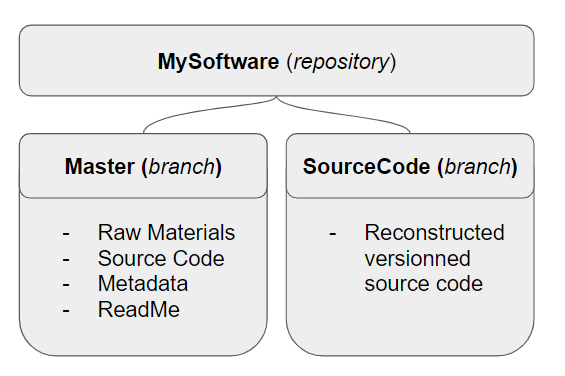
\includegraphics{./media2/01_RepoStructure.png}
\caption{Final Github repository structure.}\label{fig:repoStructure}
}
\end{figure}

\textbf{Some vocabulary} If you are not familiar with Git:

\begin{itemize}
\tightlist
\item
  A \emph{repository} is similar to a folder, a place where you can
  store your code, your files, and each file's revision history
\item
  A \emph{branch} is a parallel version of your code that is contained
  within the repository, but does not affect the primary or main branch.
\end{itemize}

\hypertarget{prepare-your-code-for-archival}{%
\subsection{Prepare your code for
archival}\label{prepare-your-code-for-archival}}

As mentionne earlier, to start the process your code needs to be in a
machine-readable format. If the code is only available in non digital
form (e.g.~printed listings), you can either transcribe it manually (see
figure 2), or use a scanner and an OCR (optical character recognition)
tool to parse it. In the example below we scanned a paper listing. The
scanner had integrated OCR function, so we could copy-past the result in
a text editor and correct the errors manually. When saving our edited
file, we made sure to correct the file extension to reflect the
programming language (in our case .pl).

\begin{figure}
\hypertarget{fig:OCR}{%
\centering
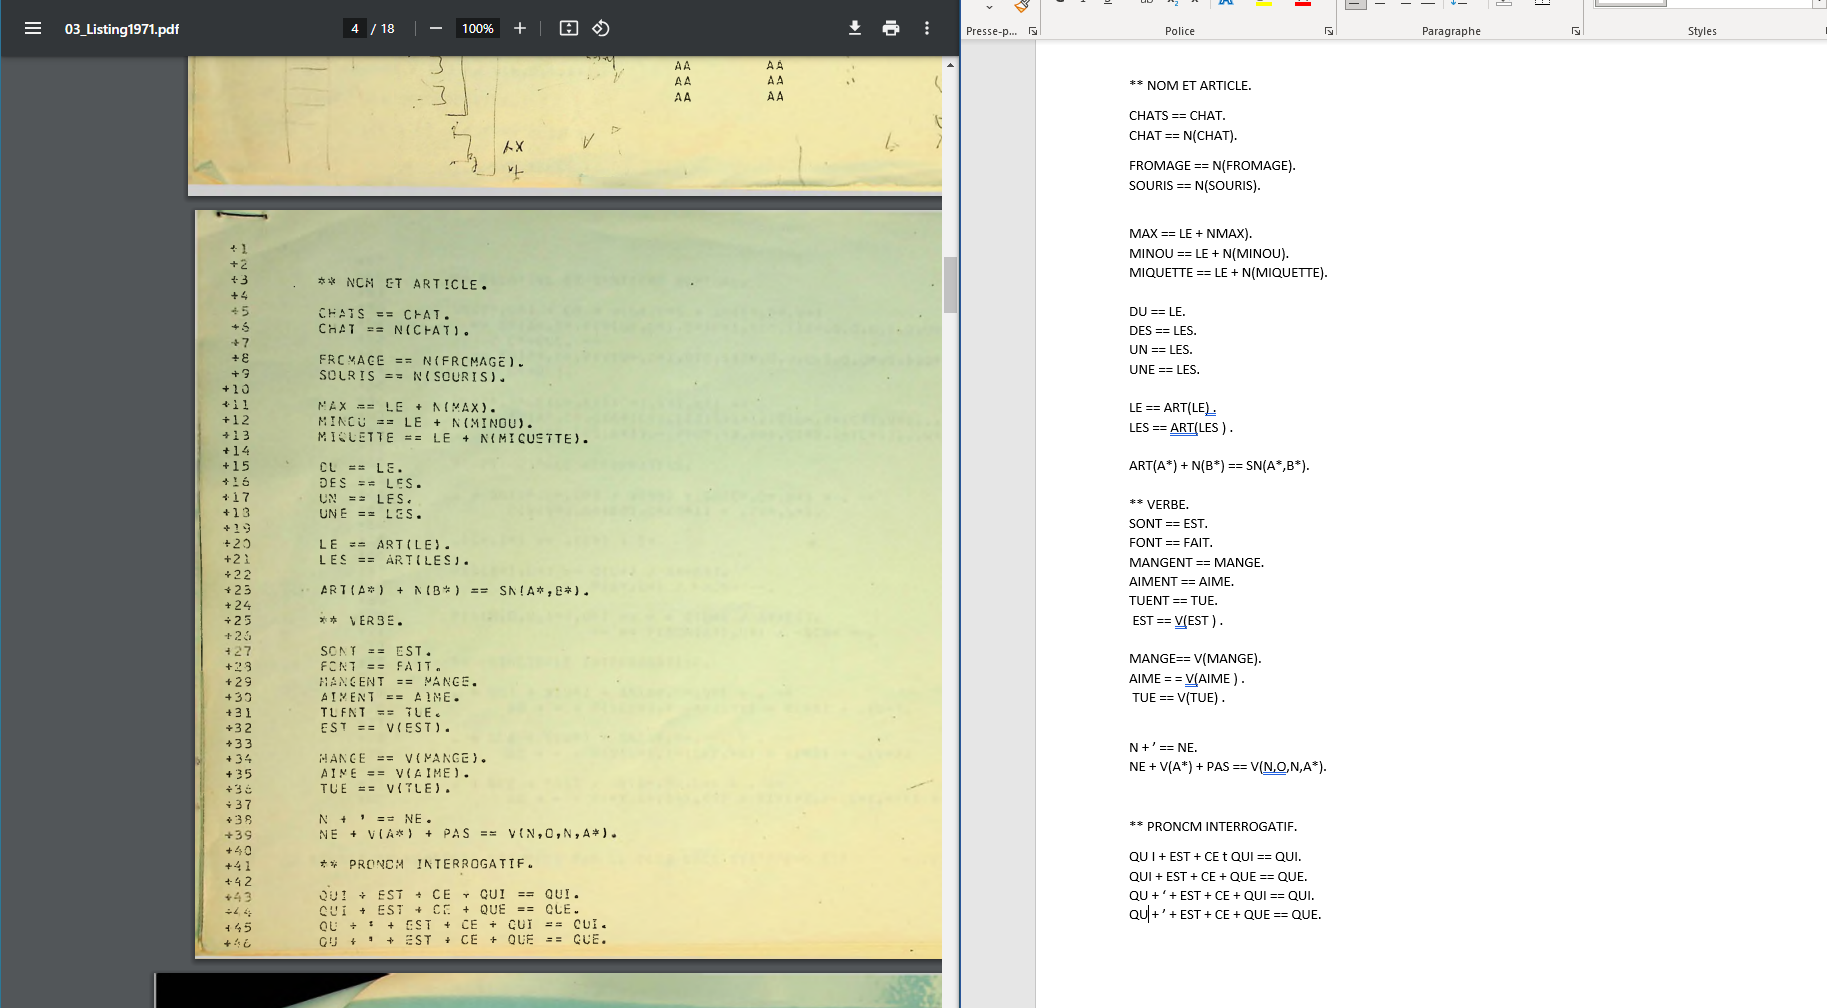
\includegraphics{./media2/09_OCR.PNG}
\caption{Make your source code machine readable.}\label{fig:OCR}
}
\end{figure}

If the raw source code is an archived and/or compressed file (.tar or
.zip), you should unpack it locally on your computer.

For historical accuracy purpose we will upload both your source code in
its initial format, and in its machine-readable format.

\hypertarget{set-up-your-working-environment}{%
\subsection{Set up your working
environment}\label{set-up-your-working-environment}}

To archive your legacy source code we will be using Github, and we
prepared a Github template that you can clone (if you are not familiar
with Github lingo \emph{to clone} means \emph{to make a copy}) to create
your own working space. Visit the template page on Github\footnote{https://github.com/mathfichen/Swhap-Template},
on the upper right hand corner click on
\passthrough{\lstinline!Use this template!} \textgreater{}
\passthrough{\lstinline!Create a new repository!} (see figure 3).

\begin{figure}
\hypertarget{fig:template}{%
\centering
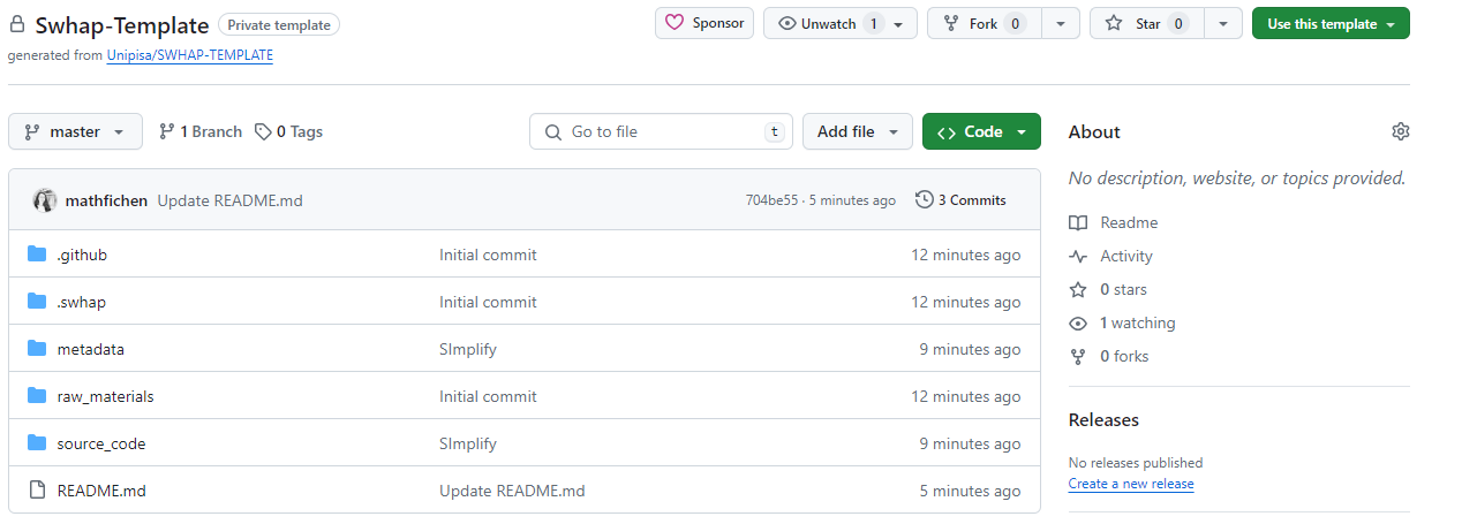
\includegraphics{./media2/01_template.png}
\caption{SWHAP template.}\label{fig:template}
}
\end{figure}

The repository you will create is a temporary working environment, and
we recommend naming it \passthrough{\lstinline!MySoftware-Workbench!}
(see figure 4), replace ``MySoftware'' by the actual name of your
software and make it private).

\begin{figure}
\hypertarget{fig:createWorkbench}{%
\centering
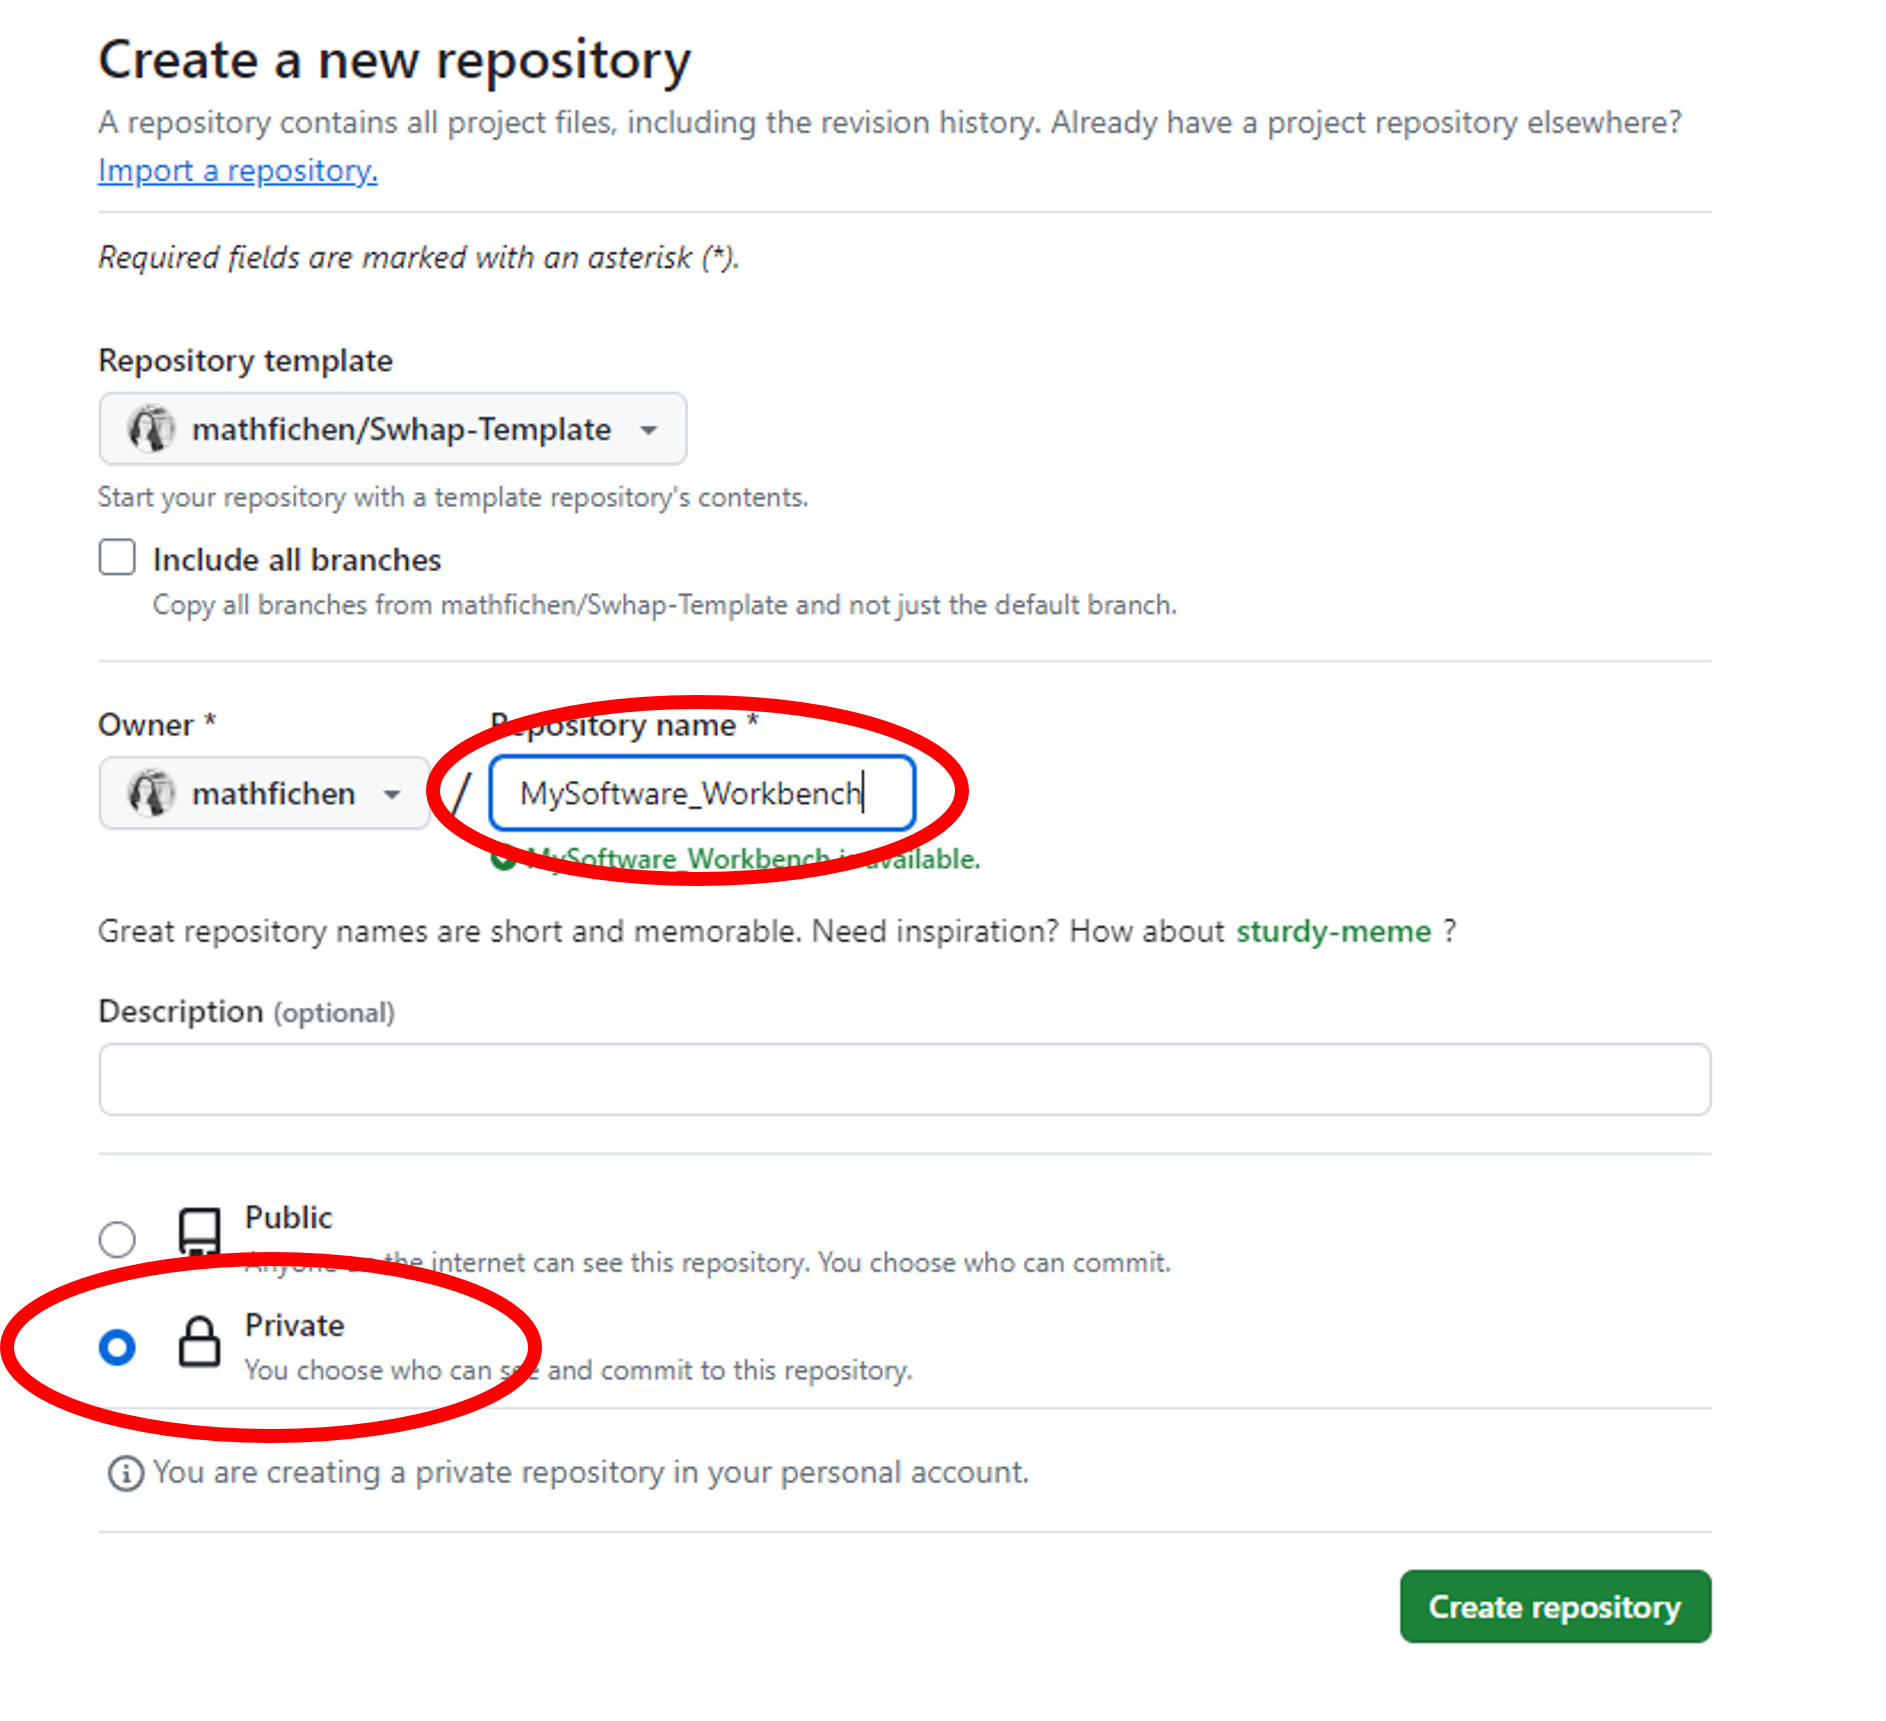
\includegraphics{./media2/02_CreateWorkbench.png}
\caption{Create your Workbench.}\label{fig:createWorkbench}
}
\end{figure}

Via the Github interface you can edit the
\passthrough{\lstinline!Read.me!} file, using the actual name of your
software. To edit a file in Github click on the pencil symbol. When you
are done editing, click on \passthrough{\lstinline!Commit!} to save your
changes.

To start working, we create a local copy on our computer, cloning this
repository. By clicking on the green button
\passthrough{\lstinline!Code!}, we get a link that we can use for this
purpose in the following command from the command line:

\begin{lstlisting}
git clone git@github.com:mathfichen/MySoftware_Workbench.git
\end{lstlisting}

This command will create local version of the Workbench on your
computer, that you can manipulate (add files, edit files, create folders
etc) the same way you would usually do it.

In our case (using Linux Subsystem for Windows), the local copy of
\passthrough{\lstinline!MySoftware\_Workbench!} has been created at this
location:

\passthrough{\lstinline!Linux!} \textgreater{}
\passthrough{\lstinline!Ubuntu!} \textgreater{}
\passthrough{\lstinline!home!} \textgreater{}
\passthrough{\lstinline!mathfichen!} \textgreater{}
\passthrough{\lstinline!MySoftware\_Workbench!}.

Open a Linux command line interpreter an navigate to
\passthrough{\lstinline!MySoftware\_Workbench!}. In our case the
interpreter current directory is
\passthrough{\lstinline!/home/mathfichen!}, so we juste type:

\begin{lstlisting}
cd MySoftware_Workbench
\end{lstlisting}

\hypertarget{upload-collected-files}{%
\subsection{Upload collected files}\label{upload-collected-files}}

You are now ready to upload your materials to the
\passthrough{\lstinline!Workbench!}. In your local Workbench, navigate
to the \passthrough{\lstinline!raw\_materials!} folder. This folder is
meant to store all your initial materials, to help any future viewer
understand the origin of the code. This covers the source code in its
initial format (scanned listing, compressed file etc.) as well as any
contextual element. For example, if the source code was sent over to you
by the historical author via email, you can also store this email. You
can also store any item you may deem relevant to understand the
historical context in which the software was produced, such as technical
documentation.

In our case we uploaded two documents: a scanned listing from 1971 and a
later digital version from 1972 in a compressed file.

\begin{figure}
\hypertarget{fig:RawMaterials_local}{%
\centering
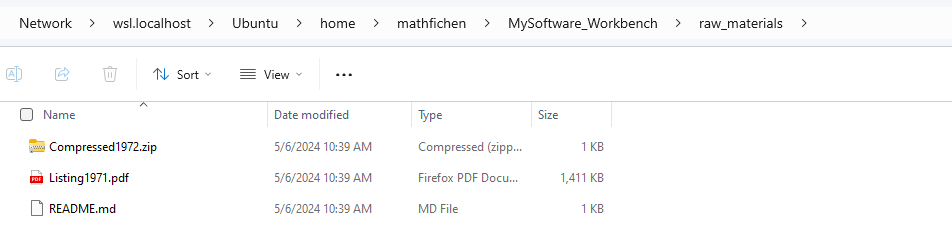
\includegraphics{./media2/12_AddRawMaterials_local.png}
\caption{Add raw materials.}\label{fig:RawMaterials_local}
}
\end{figure}

To synchronize our local Workbench with the remote repository, we run
the following command lines:

\begin{lstlisting}
git add raw_source_code
git commit -m "Added raw material"
git push
\end{lstlisting}

The resulting state of \passthrough{\lstinline!raw\_materials!} in the
remote repository is shown in Figure 5.

\begin{figure}
\hypertarget{fig:RawMaterials_local}{%
\centering
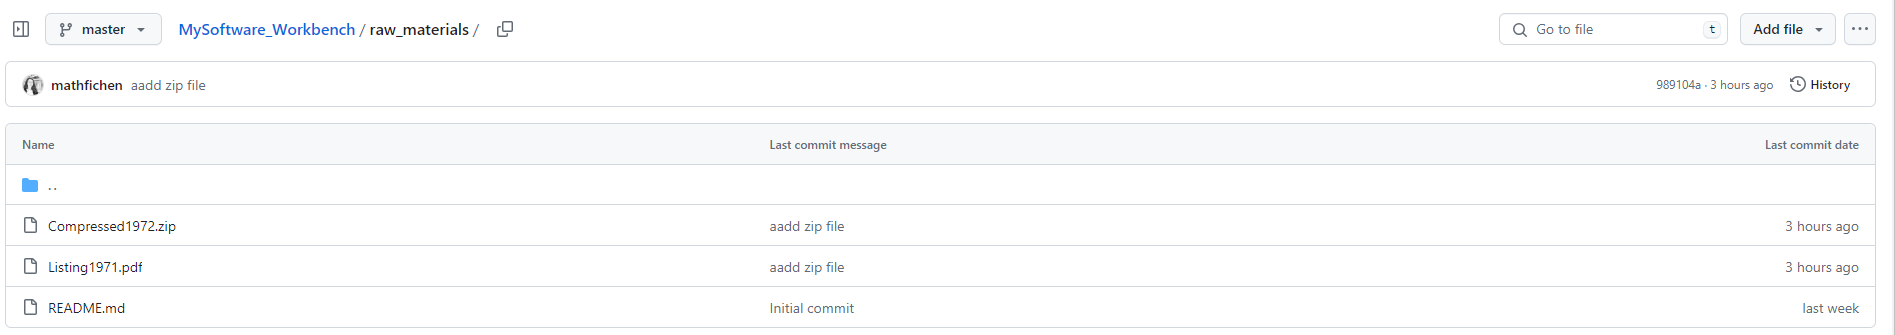
\includegraphics{./media2/13_AddRawMaterials.png}
\caption{Synch raw materials.}\label{fig:RawMaterials_local}
}
\end{figure}

\hypertarget{fill-in-the-metadata}{%
\subsection{Fill in the metadata}\label{fill-in-the-metadata}}

Then navigate to the \passthrough{\lstinline!metadata!} folder and open
the \passthrough{\lstinline!catalogue.md!} file using any text editor.
This file will help any future viewer to better understand the different
items you uploaded. Edit the file, filing in the metadata linked to each
item your uploaded.

Go back to the \passthrough{\lstinline!metadata!} folder and go to the
\passthrough{\lstinline!license.md!} file and fill in any license
information you have about the usage of the software you are archiving.

Go back once again to the \passthrough{\lstinline!metadata!} folder and
update the \passthrough{\lstinline!version-history.csv!} folder. The
content of this file should correspond to the data you will want to use
later on in the process when reconstructing the code synthetic history
(see section \emph{5.7 (Re-)Create the development History})

The CodeMeta project defines a standard JSON structure for software
metadata. This JSON will allow your code to be more easily discovered by
search engines (including the Software Heritage search engine). You can
generate such a JSON file using the CodeMeta generator\footnote{See the
  Code Meta project at https://codemeta.github.io/ and the Code Meta
  Generator at https://codemeta.github.io/codemeta-generator/}. Add this
JSON file to
\passthrough{\lstinline!MySoftware\_Workbench!}\textgreater{}\passthrough{\lstinline!Metadata!}
folder and synchronize with the distant repository.

Synchronize with the remote repository using the following command
lines:

\begin{lstlisting}
git add metadata
git commit -m "Updated metadata"
git push
\end{lstlisting}

You can see an example of the different metadata files looking at
\href{https://github.com/mathfichen/MySoftware/tree/master/metadata}{\emph{MySoftware}
final repository}

\hypertarget{upload-machine-readable-source-code}{%
\subsection{Upload machine readable source
code}\label{upload-machine-readable-source-code}}

We are now going to upload the machine readable versions of your source
code into the \passthrough{\lstinline!source\_code!} folder. Each
version of the source code should be in a machine readable format, and
stored in a dedicated sub-folder.

In our case we create two folders, \passthrough{\lstinline!v1!} and
\passthrough{\lstinline!v2!}. \passthrough{\lstinline!v1!} contains the
transcribed version of our scanned paper listing from 1971, and
\passthrough{\lstinline!v2!} contains the unzipped source code from
1972.

When you are done, synchronize with the remote repository:

\begin{lstlisting}
git add source_code
git commit -m "Added machine readable source code"
git push
\end{lstlisting}

You can check the result in the distant repository.

\begin{figure}
\hypertarget{fig:RawMaterials_local}{%
\centering
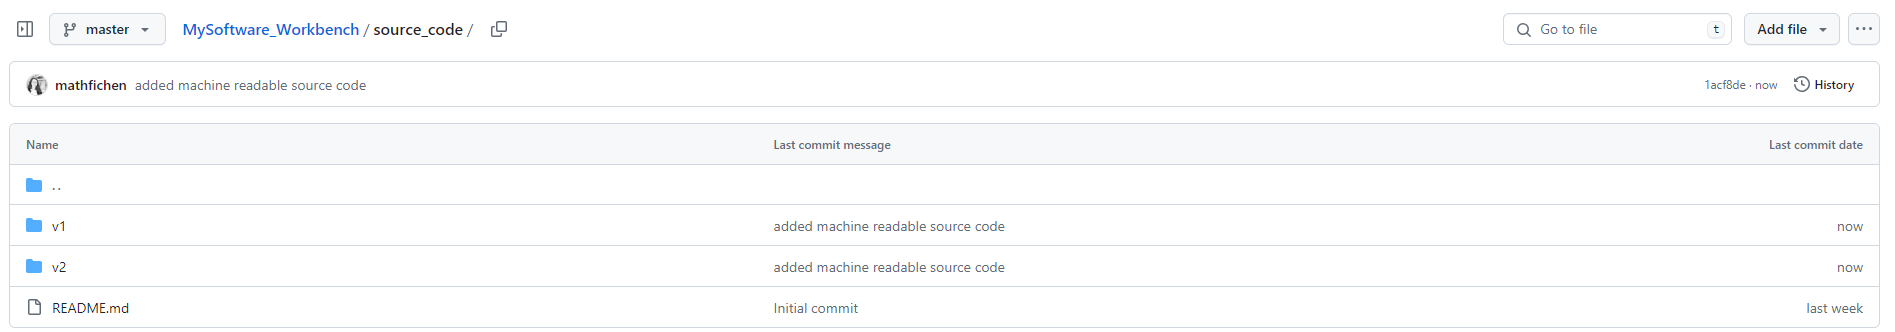
\includegraphics{./media2/14_addedSourceCode.png}
\caption{Add machine readable source
code.}\label{fig:RawMaterials_local}
}
\end{figure}

\hypertarget{re-create-the-development-history}{%
\subsection{(Re-)Create the development
History}\label{re-create-the-development-history}}

The development history can now be (re-)created either by issuing
manually (i.e.~for each version directory) the appropriate git commands,
or by using a specialized tool. This recreated development history will
be stored in a dedicated branch, that we will call
\passthrough{\lstinline!SourceCode!}. This branch will be created as an
empty orphan branch, meaning that it will be cleaned of any previous
content or commits information, as if it were a standalone branch.

\hypertarget{manually}{%
\subsubsection{Manually}\label{manually}}

We first create the SourceCode orphan branch

\begin{lstlisting}
git checkout --orphan SourceCode
\end{lstlisting}

An remove all files and folders:

\begin{lstlisting}
git rm -rf *
\end{lstlisting}

Then, for every directory of \passthrough{\lstinline!source\_code!}
containing a version of the source code, in chronological order, we copy
its contents from the \passthrough{\lstinline!master!} branch to the
\passthrough{\lstinline!SourceCode!} branch, and commit it with the
appropriate metadata, as recorded in
\passthrough{\lstinline!version\_history.csv!}.

In our case here is how we copy the source contents into our branch:

\begin{lstlisting}
git checkout master -- source_code/v1/*
mv source_code/v1/* .
rm −rf source_code
\end{lstlisting}

Then we use the following template to create manually an individual
commit/release:

\begin{lstlisting}
export GIT_COMMITTER_DATE="YYYY-MM-DD HH:MM:SS"
export GIT_COMMITTER_NAME="Commiter Name"
export GIT_COMMITTER_EMAIL="email@address"
export GIT_AUTHOR_DATE="YYYY-MM-DD HH:MM:SS"
export GIT_AUTHOR_NAME="Author Name"
export GIT_AUTHOR_EMAIL=<email@address>"
git add -A
git commit -m "Commit Message Here"
\end{lstlisting}

In our case

\begin{lstlisting}
export GIT_COMMITTER_DATE="2024-05-01 00:00:00"
export GIT_COMMITTER_NAME="Math Fichen"
export GIT_COMMITTER_EMAIL="mathfichen@monadresse.com"
export GIT_AUTHOR_DATE="1972-05-01 00:00:00"
export GIT_AUTHOR_NAME="Colmerauer et al."
export GIT_AUTHOR_EMAIL="<>"
git add -A
git commit -m "V1 of MySoftware"
\end{lstlisting}

We also need to add an annotated tag to this version. For version 1 of
MySoftware, here is the command we used, you can adapt it to your needs:

\begin{lstlisting}
git tag -a 1 -m "Version 1"
\end{lstlisting}

Finally, we clean up the directory before importing a new version

\begin{lstlisting}
    git rm -rf *
\end{lstlisting}

Redo the previous command lines for each version, starting at
\passthrough{\lstinline!git checkout master -- source\_code/v2!}. For
the last version do not clean up the directory.

Finally, synchronize with your remote repository, creating a new remote
\passthrough{\lstinline!SourceCode!} branch.

\begin{lstlisting}
git push --tags origin +SourceCode:SourceCode
\end{lstlisting}

In your distant repository you will now see a new
\passthrough{\lstinline!SourceCode!} branch, that will only display the
latest version of your code (See figure 8). The development history of
your code can be seen in the \emph{commits} history.
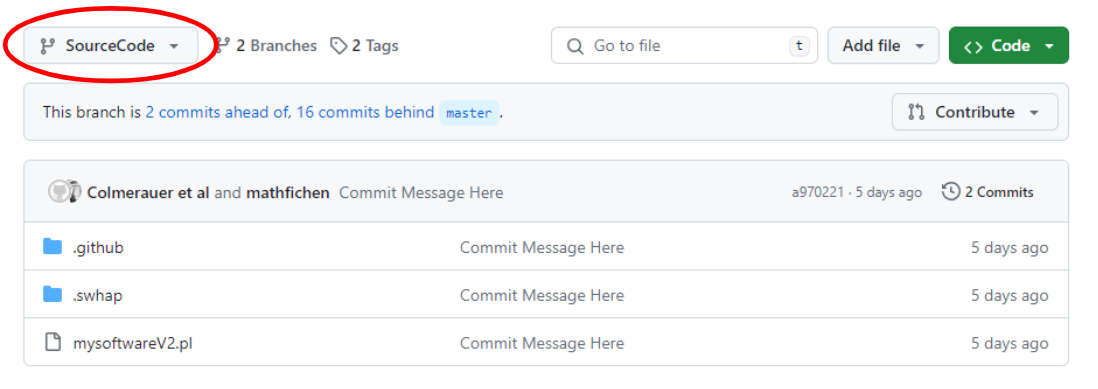
\includegraphics{./media2/15_SourceCodeBranch2.png}

\hypertarget{with-dt2sg}{%
\paragraph{With DT2SG}\label{with-dt2sg}}

If you have numerous source code versions and do not want to reconstruct
the development history by hand, the University of Pisa developped a
script to do it for you, called
\href{https://github.com/Unipisa/DT2SG}{DT2SG}. This script will
automatically used the information stored into version\_history.csv to
perform the successive commits.

Here are the associated Git instructions to run it:

\begin{lstlisting}
dotnet ./DT2SG/DT2SG_app.dll -r mathfichen/MySoftware_Workbench/source_code/ -m mathfichen/MySoftware_Workbench/metadata/version_history.csv
\end{lstlisting}

\hypertarget{create-the-final-repository}{%
\subsection{Create the final
repository}\label{create-the-final-repository}}

You are now ready to create the final public repository of your
Software, that will be ingested into the Software Heritage archive. Go
to the Github interface. From the \passthrough{\lstinline!home!} page,
click on the \passthrough{\lstinline!New!} green button and create a new
public repository, named after your software (See Figure 9).

\begin{figure}
\hypertarget{fig:FinalRepo}{%
\centering
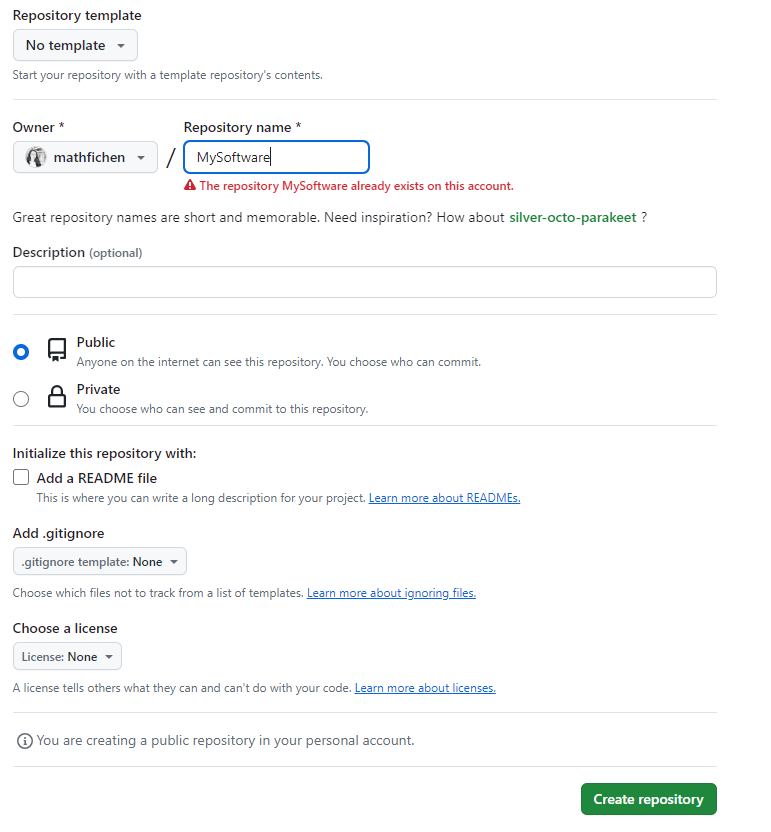
\includegraphics{./media2/17_Finalrepo.png}
\caption{Create final repository.}\label{fig:FinalRepo}
}
\end{figure}

We populate this final \passthrough{\lstinline!MySoftware!} repository
from our workbench.

\begin{lstlisting}
git push --tags git@github.com:mathfichen/MySoftware.git +master:master +SourceCode:SourceCode
\end{lstlisting}

To facilitate the search of the created repository, add the
``software-heritage'', ``legacy code'', ``archive'' and ``swhap'' topic
tags to your repository. To do so, click on the
\passthrough{\lstinline!setting!} icon of your repository and add the
relevant topics (See figure 10).

\begin{figure}
\hypertarget{fig:Topics}{%
\centering
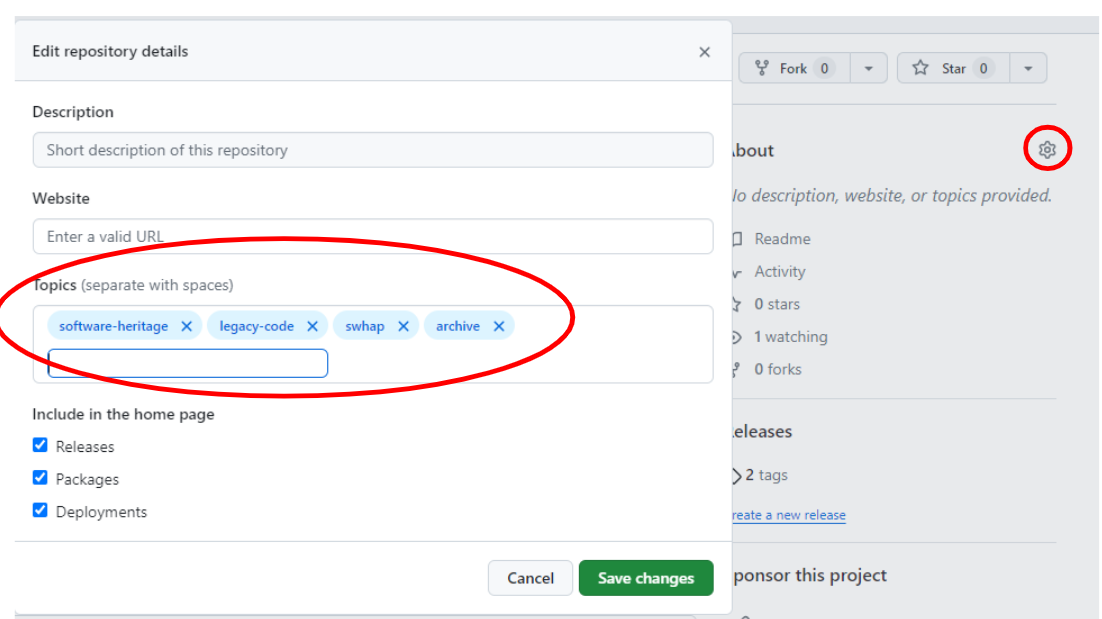
\includegraphics{./media2/18_tags.png}
\caption{Add topics.}\label{fig:Topics}
}
\end{figure}

\hypertarget{sec:archive}{%
\section{Trigger the Software Heritage Acquisition}\label{sec:archive}}

Even though Software Heritage automatically archives any repository
publicly available on Github we suggest yout to specifically schedule it
to make sure everything runs smoothly. To do so, visit the Software
Heritage ``Save code now'' page\footnote{https://archive.softwareheritage.org/save/},
and submit the URL of your software final repository.

\begin{figure}
\hypertarget{fig:saveCodeNowURL}{%
\centering
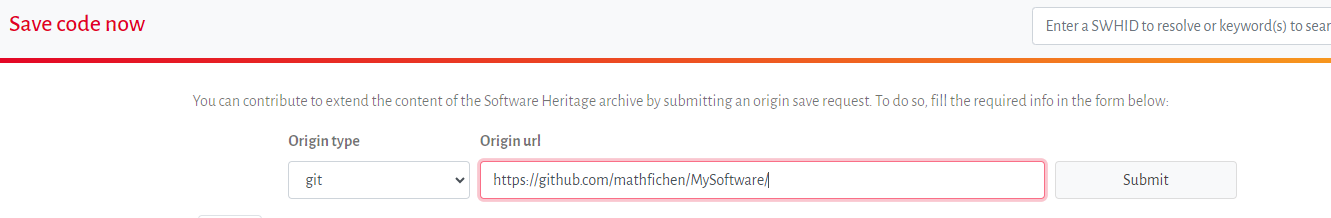
\includegraphics{./media2/19_savecode.png}
\caption{View of the \emph{Save Code Now} URL entry
bar}\label{fig:saveCodeNowURL}
}
\end{figure}

You can then follow the archival status of your code in the \emph{Browse
Save Request} tab below\footnote{https://archive.softwareheritage.org/save/list/}.

Your legacy code is now forever safely archived on the Software Heritage
universal archive. You can search for its archive location using its URL
in Software Heritage\footnote{https://archive.softwareheritage.org/browse/search/}.
Your code now has a unique identifier called \emph{SWHID}\footnote{See
  https://docs.softwareheritage.org/devel/swh-model/persistent-identifiers.html
  for more information on the SWHID} (Software Heritage IDentifier),
that can be used for example to cite your code in an academic paper.
This \emph{SWHID} can be found clicking on the
\passthrough{\lstinline!Permalink!} tab on the right side of your
archived code page.

Also on the \passthrough{\lstinline!Permalink!} tab, you can click on
the two \passthrough{\lstinline!archived!} badges and retrieve a
markdown code snippet. Use these code snippets in the README of your
final software repository. This will display the badges on the first
page of your repository, allowing anyone visiting it to click on them
and get access to its archive on Software Heritage (See figure 12).

\begin{figure}
\hypertarget{fig:badge}{%
\centering
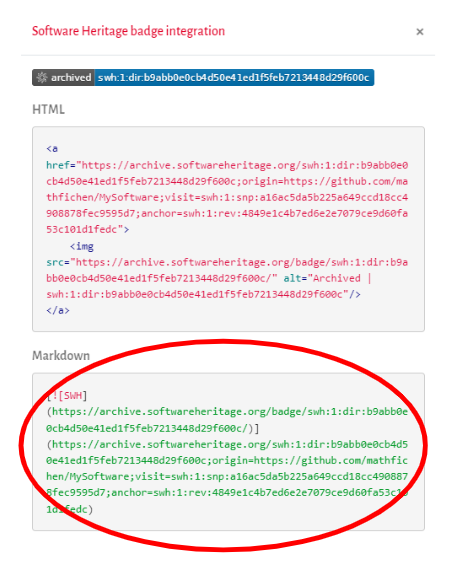
\includegraphics{./media2/20_SWHbadges.png}
\caption{View of the \_Permalink\_tab}\label{fig:badge}
}
\end{figure}

\hypertarget{congrats}{%
\subsubsection{Congrats}\label{congrats}}

Congrats, you are done archiving your code! Please do not hesistate to
share your thoughts and send us feedback using the
\href{https://sympa.inria.fr/sympa/subscribe/swhap-inria?previous_action=info}{mailing
list}).

\printbibliography

\end{document}
